\documentclass{beamer}

\usepackage[british]{babel}
\usepackage{graphicx,hyperref,ru,url}
\usepackage{amsmath}
\usepackage{amssymb}
\newcommand{\R}{\mathbb{R}}
\usepackage{adjustbox} % Shrink stuff
% Fancy fit image command with optional caption
\makeatletter
\newcommand{\fitimage}[2][\@nil]{
	\begin{figure}
		\begin{adjustbox}{width=0.9\textwidth, totalheight=\textheight-2\baselineskip-2\baselineskip,keepaspectratio}
			\includegraphics{#2}
		\end{adjustbox}
		\def\tmp{#1}%
		\ifx\tmp\@nnil
		\else
		\caption{#1}
		\fi
	\end{figure}
}
% RU style for Beamer
% The title of the presentation:
%  - first a short version which is visible at the bottom of each slide;
%  - second the full title shown on the title slide;
\title[Make Use of NN for Solving PDEs]{
  Make Use of Neural Networks for Solving Partial Differential Equations\\(The Deep Ritz Method)}

% Optional: a subtitle to be dispalyed on the title slide
\subtitle{Institute for Advanced Studies in Basic Sciences}

% The author(s) of the presentation:
%  - again first a short version to be displayed at the bottom;
%  - next the full list of authors, which may include contact information;
\author[Sajed N. Zarrinpour]{
  Sajed N. Zarrinpour \\\medskip
  {\small \url{sa.zarrinpour@iasbs.ac.ir}} \\ 
  {\small \url{http://www.iasbs.ac.ir/~sa.zarrinpour}}}

% The institute:
%  - to start the name of the university as displayed on the top of each slide
%    this can be adjusted such that you can also create a Dutch version
%  - next the institute information as displayed on the title slide
\institute[Institute for Advanced Studies in Basic Sciences]{
  Math Department -- Numerical Analysis \\
  Institute for Advanced Studies in Basic Sciences}

% Add a date and possibly the name of the event to the slides
%  - again first a short version to be shown at the bottom of each slide
%  - second the full date and event name for the title slide
\date[\today]{
  Fall 2019 }

\begin{document}

\begin{frame}
  \titlepage
\end{frame}

\begin{frame}
  \frametitle{Outline}

  \tableofcontents
\end{frame}

% Section titles are shown in at the top of the slides with the current section 
% highlighted. Note that the number of sections determines the size of the top 
% bar, and hence the university name and logo. If you do not add any sections 
% they will not be visible.
\section{Introduction}

\begin{frame}
  \frametitle{Introduction}
	Numerical Methods!
  \begin{itemize}
    \item <1- > Why?
    \item <2- > Why Not?
    \item <3- > Cheat?
    \item <4- > Lets get into it!
  \end{itemize}
\end{frame}

\section{Background information}

\begin{frame}
  \frametitle{Finite Element Method}

  \begin{block}{Poisson Equation on Unit Square - Strong Form}
    \begin{equation*}
    	\begin{cases}
    	 -\Delta u = f (x)\hspace{50pt} ,on \Omega = [0\times 1] \times [0\times 1]  
    	 \\
    	 u = 0 \hspace{80pt} ,on \partial \Omega
    	\end{cases}	
    \end{equation*}
  \end{block}

\end{frame}

\begin{frame}
	\frametitle{Finite Element Method}	
	\begin{block}{Poisson Equation on Unit Square - Weak Form}		
		$\sum_{i=1}^{M} c_i <\phi_i,\phi_j> = <f,\phi_j> \hspace{30pt} i=1,...,M,$		
		\\where\\	
		 $u_h = \sum_{i=1}^{M} c_i \phi_i \hspace{5pt} and \in V_h=span\{\phi_i\}_{i=1}^{M}$		
	\end{block}	
\end{frame}

\begin{frame}
	\frametitle{Finite Element Method}
	
	\textbf{Quite Complex eh?}\centering\\
	\textit{Lets cheat!}\centering\\
	
\end{frame}

\section{Problem Definition}
\begin{frame}
	\frametitle{Deep Ritz Method}
	
	\begin{block}{Universal Approximation Theorem}
		Let $\phi:\R \to \R$ be a nonconstant, bounded, and continuous function. Let $I_m$ denote the m-dimensional unit hypercube $[0 \times 1]^m$. The space of real-valued continuous functions on $I_m$ is denoted by $C(I_m)$. Then, given any $\epsilon >0$ and any function $f \in C(I_m)$, there exist an integer N, real constants $v_i, b_i \in \R$ and real vectors $w_i \in \R^m$ for i=1,...,N, such that we may have define :
		
		$F(x) = \sum_{i=1}^{N} v_i \phi(w_{i}^{T}x + b_i)$
		as an approximate realization of the function f; that is,
		$|F(x)-f(x)| < \epsilon$
		for all $x\in I_m$. 		
	\end{block}	
\end{frame}

\begin{frame}
	\frametitle{Deep Ritz Method}
	
	\begin{block}{Poisson Equation - Neural Networks Form}
		\fitimage[Autoscaling image]{DRM.png}
	\end{block}	

\end{frame}

\begin{frame}
	\frametitle{Deep Ritz Method}
	
	\begin{block}{Poisson Equation - Neural Networks Form}
	$u_{\theta}(x) = a . f_{n}(x) \circ ... \circ f_{1}(x) +b$ \\
	where \\
	$f_{i}(x) = \phi(W_i2 . \phi(W_i1 . x + b_{i1}) + b_{i2}) + x $ and $a \in \R^m, b\in\R $ \\
	and $\phi(x) = \max\{x^3,0\}$
	\end{block}	
\end{frame}




\section{Results}

\begin{frame}
	\frametitle{Deep Ritz Method}
	\begin{figure}
		\caption{(a) DRM - 811 parameter, (b) FDM - 1681 parameter}
		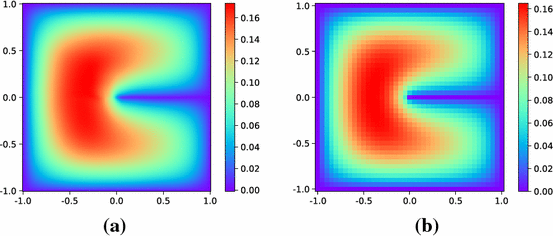
\includegraphics[width=\textwidth,height=\textheight,keepaspectratio]{DRMvsFDM.png}

	\end{figure}
\end{frame}


\section{Conclusion}
\begin{frame}
	\frametitle{Conclusion}
	\begin{itemize}
		\item <1- > calculation of the basis
		\item <2- > better accuracy
	\end{itemize}
\end{frame}

\begin{frame}
  \frametitle{Q\&A}
\textbf{"Ask, and it shall be given you!"}\centering\\
\em Matthew 7:7
\end{frame}
\section{References}
\begin{frame}
	\begin{itemize}
		\item \href{https://arxiv.org/pdf/1710.00211.pdf}{The Deep Ritz Method}
		\item \href{https://en.wikipedia.org/wiki/Universal_approximation_theorem}{Universal Approximation Theorem}
	\end{itemize}
\end{frame}

\end{document}
